\documentclass[11pt]{report}

\special{papersize=8.5in,11in}

\topmargin -0.5in \oddsidemargin 0.00in \evensidemargin 0.00in
\textwidth 6.75in \textheight 9.0in \headheight 0.25in \headsep
0.25in \footskip 0.5in \hoffset 0in \marginparpush 0.0in
\marginparwidth 0.0in \marginparsep 0.2in

\setcounter{page}{1}

\newcommand{\D}{\displaystyle}\newcommand{\T}{\textstyle}
\newcommand{\e}{{\mathrm{exp}}}
\newcommand{\dd}{{\mathrm d}}
\newcommand{\comment}[1]{}
\newcommand{\mb}{\mathbf}
\reversemarginpar

\usepackage[final]{graphicx}
\usepackage{fancyhdr}
%\graphicspath{{Papers/}}
\usepackage{amsthm,amssymb,amsmath}
\usepackage{cite}
\usepackage{geometry}
\usepackage{amsmath}
\usepackage{booktabs}
\usepackage{color}
\usepackage{setspace}
\usepackage{subfigure}
\usepackage{url}
%\usepackage[top=2.5cm, bottom=2.5cm, right=3.5cm, left=3.5cm]{geometry}
\geometry{a4paper,scale=0.8}
\setcounter{secnumdepth}{3}

\title{Research Progress Report}

\author{Botao Zhu}

\begin{document}
	
	\maketitle
	\lhead{\sf Research Progress Report-5th} \chead{} \rhead{\sf Botao Zhu}
	\lfoot{CTRG, University of Saskatchewan} \cfoot{} \rfoot{Page \thepage}
	\renewcommand{\footrulewidth}{1.0pt}
	\renewcommand{\headrulewidth}{2.0pt}
	\renewcommand{\arraystretch}{1.3}
	\pagestyle{fancy}
	
	\renewcommand{\thesection}{\arabic{section}}
	
	\section{Reading and Research Activities}
	
	\subsection{Reading Summary}
	
	
	\noindent Fractional Fourier transform(FRFT) is a generalization of the ordinary Fourier transform (FT), which has been widely used in signal processing and image processing. The output of FRFT with different orders represents mixed time and frequency components of signal. \cite{8492732} constructs a complex-valued fractional Fourier transform matrix to transform input layer data for obtaining real-valued coefficients of fractional transform. The real-valued output of fractional transform can be worked as the new input layer of classifier. However, this way is still in real domain.\\
	
    \noindent Recent work on recurrent neural networks and older fundamental theoretical analysis suggests that complex numbers have a richer representational capacity. The role of representations based on complex numbers has started to receive increased attention because easier optimization, better generalization characteristics, faster learning,etc.  \cite{DBLP:journals/corr/TrabelsiBSSSMRB17} has explored a wide variety of complex convolutional network architectures, it provides the key atomic components for complex-valued deep neural networks. Its contributions are as follow:\\
    1. A formulation of complex bath normalization.\\
    2. Complex-valued ReLU-based activation function.\\
    3. Complex weight initialization.
    \begin{itemize}
    	\item \textbf{Complex convolution}\\
    	In order to perform convolution in the complex domain, they convolve a complex filter matrix $\mathbf{W} = \mathbf{A}+i\mathbf{B}$ by a complex vector $\mathbf{h} = \mathbf{x}+i\mathbf{y}$ where $\mathbf{A}$ and $\mathbf{B}$ are real matrices and $\mathbf{x}$ and $\mathbf{y}$ are real vectors. Convolving the vector $\mathbf{h}$ by the filter $\mathbf{W}$,
    	\begin{equation}
    	\mathbf{W} * \mathbf{h} = \left(\mathbf{A} * \mathbf{x}-\mathbf{B} * \mathbf{y}\right) + i\left(\mathbf{B} * \mathbf{x} + \mathbf{A} * \mathbf{y}\right)
    	\end{equation}
    \end{itemize}
    
    \begin{itemize}
    	\item \textbf{Complex bath normalization}\\
    	 The complex bath normalization is defined as:
    	 \begin{equation}
    	 \text{BN}\left(\widetilde{\mathbf{x}}\right) = \gamma \widetilde{\mathbf{x}} + \beta
    	 \end{equation}
    	 $\widetilde{\mathbf{x}}$ is the normalized input input with real and imaginary variance 1. 
    	 \begin{equation}
    	 \widetilde{\mathbf{x}} = \left(\mathbf{V}\right)^{-\frac{1}{2}}\left(\mathbf{x}-E[\mathbf{x}]\right)
    	 \end{equation}
    	 $\mathbf{V}$ is $2 \times 2$ covariance matrix\\
    	 \begin{equation}
    	 \mathbf{V} = \begin{pmatrix}
    	 V_{rr} &V_{ri} \\
    	 V_{ir} &V_{ii}
    	 \end{pmatrix}
    	 \end{equation}
    	 The mean subtraction and multiplication by the inverse square root of the variance ensures that $\widetilde{\mathbf{x}}$ has standard complex distribution with 0 mean and 1 covariance.\\
    	 The shift parameter $\beta$ is a complex parameter with the real and imaginary means. The scaling parameter $\gamma$ is a $2 \times 2$ positive semi-definite matrix with only three degrees of freedom.
    	 \begin{equation}
    	 \gamma = \begin{pmatrix}
    	 \gamma _{rr} &\gamma _{ri} \\
    	 \gamma _{ri} &\gamma _{ii}
    	 \end{pmatrix}
    	 \end{equation}
    	 
    \end{itemize}
    
    \begin{itemize}
    	\item \textbf{Complex-valued ReLU-based activation function}\\
    	Numerous activation functions have been proposed in the literature in order to deal with complex-valued representations. \cite{DBLP:journals/corr/ArjovskySB15} defines a kind of activation functions
    	\begin{equation}
    	\text{modReLU}(\mathnormal{z}) = \text{ReLU}(|\mathnormal{z}|+b)e^{i\theta_\mathnormal{z}} = \begin{cases}
    	(|\mathnormal{z}|+b)\frac{\mathnormal{z}}{|\mathnormal{z}|}, & \text{if} |\mathnormal{z}| + b \geqslant 0,\\
    	0, &\text{otherwise},
    	\end{cases}
    	\end{equation}
    	where $\theta_\mathnormal{z}$ is the phase of $\mathnormal{z}$, and $b\in \mathcal{R}$.
    \end{itemize}
    
    \begin{itemize}
    	\item \textbf{Complex weight initialization}\\
    	A complex weight has a polar form and a rectangular form
    	\begin{equation}
    	W = |W|e^{i\theta} = \mathcal{R}\{W\}+i\mathcal{L}\{W\}
    	\end{equation}
    	where $\theta$ and $|W|$ are respectively the phase and magnitude of $W$.
    	Variance can de defined as:
    	\begin{equation}
    	Var(W) = E[WW^*] - (E[W])^2 = E[|W|^2] - (E[|W|])^2
    	\end{equation}
    	Since the magnitude of complex normal values, $|W|$, is a Rayleigh distribution.
    	\begin{equation}
    	Var(|W|) = E[|W||W|^*]-(E[|W|])^2 = E[|W|^2]-(E[|W|])^2
    	\end{equation}
    	and we can have
    	\begin{equation}
    	Var(W) = Var(|W|) + (E[|W|])^2
    	\end{equation}
    	The mean and variance of Rayleigh distribution are respectively
    	\begin{equation}
    	E[|W|] = \sigma \sqrt{\frac{\pi}{2}}
    	\end{equation}
    	\begin{equation}
    	Var(|W|) = \frac{4-\pi}{2}\sigma^2
    	\end{equation}
    	Thus, the variance of $W$
    	\begin{equation}
    	Var(W) = \frac{4-\pi}{2}\sigma ^2 + \left(\sigma \sqrt{\frac{\pi}{2}}\right)^2 = 2 \sigma^2
    	\end{equation}
    	The magnitude of the complex $W$ is initialized by Rayleigh distribution with the appropriate mode $\sigma$. The variance of $W$ depends on its magnitude and not on its phase. So the phase can be initialized by uniform distribution between $-\pi$ and $\pi$. 
    \end{itemize}
	\begin{itemize}
		\item Complex convolutional residual network\\
		In deep convolutional residual network, there are several residual blocks. The residual blocks of real and complex component are shown as below.
		\begin{figure}[h!]
			\centering
			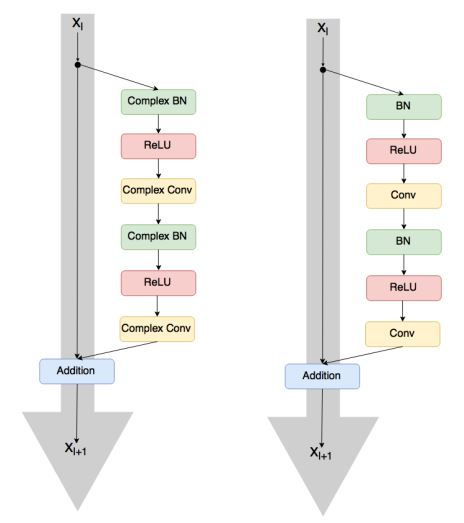
\includegraphics[width=0.4\linewidth]{residualnetwork.jpg}
			\caption{A complex convolutional residual network and an equivalent real-valued residual network}
			\label{}
		\end{figure}
		
		Since all datasets have real-valued inputs, a way to learn the imaginary components to let the rest of the network operate in the complex plane is proposed. The initial imaginary component of input by performing the operations present within a single real-valued residual block.
		\begin{equation*}
		BN -> ReLU -> Conv -> BN -> ReLU -> Conv
		\end{equation*}
	\end{itemize}
    
    At present, there are few studies on complex neural networks. So, this field is very attractive and interesting. For the future research, the first step is to plan to extend the application of complex neural networks to wireless networks. Since \cite{DBLP:journals/corr/TrabelsiBSSSMRB17}'s work is still  based on linear transformation, the second step, I plan to study complex neural networks from non-linear perspective.
    
	
	
	\section{Objectives for the Next 2 Weeks}
	\subsection{Reading} 
	Read articles in complex deep Learning.\\
	Review complex number.
	
	
	\section{Advisor's Comments}
	
	\bibliographystyle{IEEEtran}
	\bibliography{janbib}
	
\end{document}